\subsection{Sintaxis de la notación}

Partiendo de esto, lo siguiente que se realizó fue la definición de la sintaxis de la notación a usar, basados en lo definido por el metamodelo. Para esto, se decidió usar \texttt{YAML}, un lenguaje de serialización de datos orientado a la legibilidad, reconocido y usado principalmente para la creación de archivos de configuración \cite{YAML2023}. 

La sintaxis, como puede observarse en la figura \ref{fig:rail-base}, se compone de 2 partes: \texttt{Application}, donde se declara la aplicación; y \texttt{Locations}, en donde se define el contexto geográfico al igual que las necesidades de datos de estas.

\begin{figure}[H]
    \centering
    \caption{Diagrama de rail de la sintaxis definida para la notación de SmartCampusADL}
    \label{fig:rail-base}
    \vspace{2mm}
    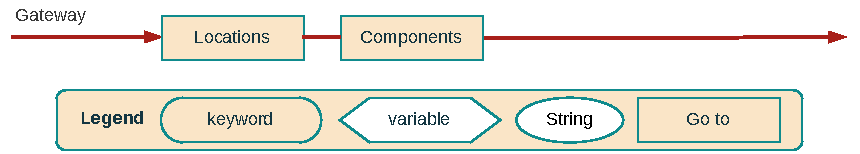
\includegraphics[width=\linewidth]{images/Railroad Base.pdf}
\end{figure}

Esta primera parte, como puede observarse en la figura \ref{fig:rail-app} se refiere al nombre que se usará para referirse a la aplicación al rededor de todos los servicios, y una descripción opcional con fines de documentación.

\begin{figure}[H]
    \centering
    \caption{Diagrama de rail de la sintaxis de declaración de la aplicación}
    \label{fig:rail-app}
    \vspace{2mm}
    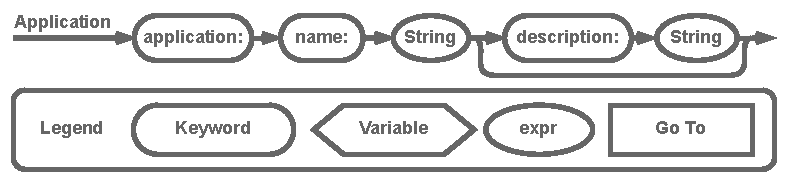
\includegraphics[width=\linewidth]{images/Railroad Application.pdf}
\end{figure}

Para especificar las \texttt{locaciones} dentro del contexto de la aplicación, se definió la sintaxis que puede observarse en la figura \ref{fig:rail-location}. Partiendo de la locación raíz de la aplicación, podrán declararse \textit{n} cantidad de locaciones, cada una con un nombre diferente.

\begin{figure}[H]
    \centering
    \caption{Diagrama de rail de la sintaxis definida para la notación del contexto geográfico de la aplicación}
    \label{fig:rail-location}
    \vspace{-2mm}
    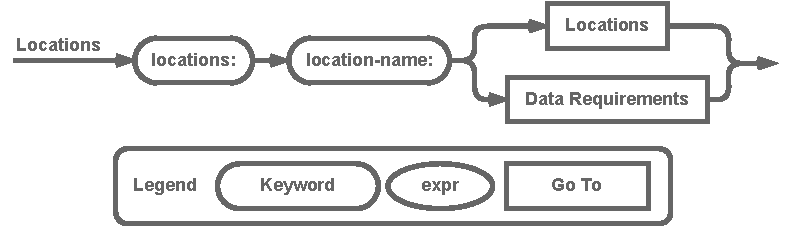
\includegraphics[width=\linewidth]{images/Railroad Locations Alt.pdf}
\end{figure}

Las locaciones pueden funcionar de una de dos maneras. La primera es como agrupadores de otras locaciones, que puede verse como varios edificios de un campus o como varios pisos de un edificio, dependiendo de la granularidad que requiera la aplicación. Y, la segunda son puntos de origen de datos requeridos por la aplicación, reportados por diversas clases de dispositivos presentes.

Los requerimientos de datos, como se puede ver en la figura \ref{fig:rail-data-req}, están compuestos de varias partes. Las \texttt{data-key} se refieren al nombre del requerimiento de dato de la locación. Se espera que estos sean los mismos usados en la parte de \texttt{values} vista en los mensajes de la plataforma Smart Campus de la figura \ref{fig:jsonSCU}.

\begin{figure}[H]
    \centering
    \caption{Diagrama de rail de la sintaxis definida para la notación de los componentes de la aplicación}
    \label{fig:rail-data-req}
    \vspace{-2mm}
    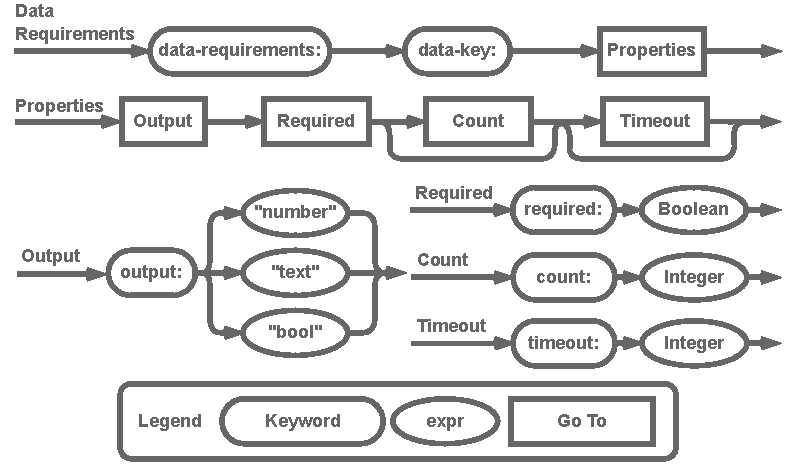
\includegraphics[width=\linewidth]{images/Railroad Data Requirements.pdf}
\end{figure}

A continuación, se procedería a definir las propiedades de dicho requerimiento de datos. Para esta primera versión de la notación, se han establecido las 4 cuatro propiedades vistas en el modelo (ver figura \ref{fig:metamodelo}), dos son obligatorias para la declaración. La primera es \texttt{output}, que hace referencia al tipo de dato esperado \footnote{Este output, en el modelo es el \textit{enum} \texttt{IoTOutput}, que representa los tipos de datos.}, y la segunda es \texttt{required}, que especifica si el requerimiento es obligatorio u opcional. Las otras dos propiedades opcionales: \texttt{count}, que representa la cantidad de fuentes de datos necesarias en la ubicación, y \texttt{timeout}, que indica el tiempo máximo entre los informes de datos. En ambos casos, de no declararlas, se tomaría como valor por defecto 0.

El resultante de esta notación serían archivos de declaración de arquitecturas, en formato YAML, similares a la que se puede observar en la figura \ref{fig:YAML-ADL}.

\begin{figure}[H]
    \centering
    \caption{YAML de una posible aplicación de monitorio}
    \label{fig:YAML-ADL}
    \begin{tabular}{c}
        \setstretch{1}
        \small
        \lstinputlisting[language=YAML]{metamodel/modelV2.yaml}
    \end{tabular}
\end{figure}

Con esto hemos creado un marco sólido para representar las aplicaciones de Smart Campus UIS. Este enfoque bien definido nos permitirá avanzar en el desarrollo de nuestras funcionalidades de comparación de los modelos, y la implementación de los mecanismos de adaptación a usar. 